%==============================================================================
% Sjabloon poster bachproef
%==============================================================================
% Gebaseerd op document class `a0poster' door Gerlinde Kettl en Matthias Weiser
% Aangepast voor gebruik aan HOGENT door Jens Buysse en Bert Van Vreckem

\documentclass[a0,portrait]{hogent-poster}
\usepackage{xcolor}

% Info over de opleiding
\course{Bachelorproef}
\studyprogramme{toegepaste informatica}
\academicyear{2025-2026}
\institution{Hogeschool Gent, Valentin Vaerwyckweg 1, 9000 Gent}

% Info over de bachelorproef
\title{Ontwikkeling en evaluatie van een proof-of-concept interface voor het efficiënt beoordelen van de toegankelijkheid van Vlaamse huisartsenpraktijken.}
\author{Neal Debot}
\email{Neal.Debot@student.hogent.be}
\supervisor{Benjamin Vertonghen}
\cosupervisor{Sabien  Van Rampelberg}

% Indien ingevuld, wordt deze informatie toegevoegd aan het einde van de
% abstract. Zet in commentaar als je dit niet wilt.
\specialisation{Full stack developer}
\keywords{toegankelijkheid huisartsenpraktijken, proof-of-concept, gezondheidszorg IT}
\projectrepo{https://github.com/NealDebot/BP-POC-Monorepo}

\begin{document}

\maketitle

\begin{abstract}
De toegankelijkheid van Vlaamse huisartsenpraktijken wordt geëvalueerd aan de hand van uitgebreide indicatorensets, 
maar dit proces wordt in de praktijk als tijdrovend en complex ervaren. 
In deze bachelorproef werd een proof-of-concept webapplicatie ontwikkeld die het evaluatieproces gebruiksvriendelijker en efficiënter maakt, 
geëvalueerd door 12 medewerkers uit huisartsenpraktijken. 
De resultaten tonen een gemiddelde SUS-score van 73,96 en een mediane invultijd van 2 minuten en 28 seconden, 
wat aantoont dat een gerichte digitale interface een belangrijke stap kan zijn richting efficiëntere toegankelijkheidsevaluaties.
\end{abstract}

\begin{multicols}{2} % This is how many columns your poster will be broken into, a portrait poster is generally split into 2 columns

\section{Introductie}
\subsection{Probleemstelling}
 
De toegankelijkheid van Vlaamse huisartsenpraktijken wordt beoordeeld aan de hand van een wetenschappelijk onderbouwde set van \textbf{38 toegankelijkheidsindicatoren}. 
De praktische toepassing ervan stuit echter op een aantal structurele knelpunten:
 
\begin{itemize}
  \item Tijdsintensief invulproces voor praktijkmedewerkers
  \item Inconsistente interpretatie van indicatoren
  \item Moeilijk toegankelijke en onoverzichtelijke feedback
\end{itemize}
 
Er bestaat bijgevolg een concrete nood aan een digitale oplossing die zowel het invullen vereenvoudigt als de terugkoppeling van resultaten toegankelijker maakt.

\subsection{Doelstelling}

Het doel van deze bachelorproef is het ontwikkelen en evalueren van een proof-of-concept webapplicatie die:
 
\begin{itemize}
  \item Vragenlijsten vereenvoudigt en digitaliseert
  \item Praktijkgegevens centraal opslaat en hergebruikt
  \item Feedback over toegankelijkheid overzichtelijk en toegankelijk maakt
\end{itemize}
 
\subsection{Onderzoeksvraag}
 
\textit{In welke mate kan een digitale interface toegankelijkheidsevaluaties sneller en gebruiksvriendelijker maken voor Vlaamse huisartsenpraktijken?}
 
\section{Methodologie}

Het ontwikkeltraject verliep in vijf opeenvolgende fasen:

\begin{center}
  \captionsetup{type=figure}
  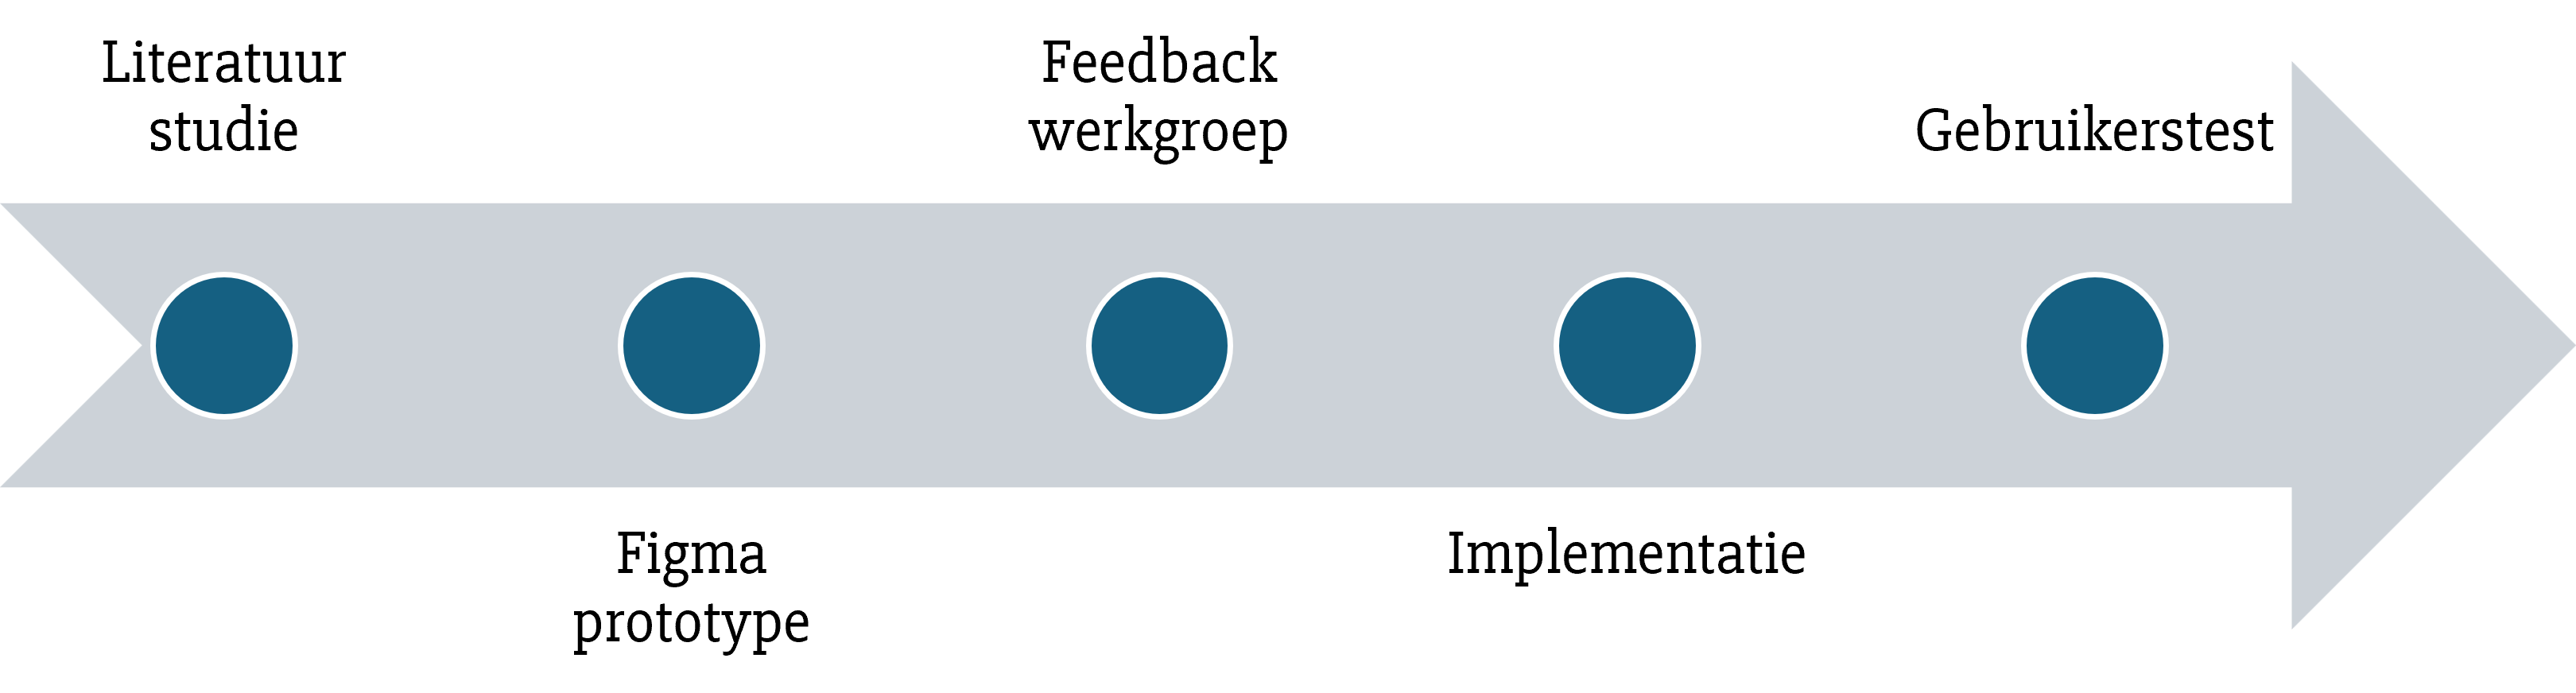
\includegraphics[width=1.0\linewidth]{graphics/Tijdlijn.png}
  \captionof{figure}{Ontwikkeltraject van de proof-of-concept}
\end{center}
 
De usability werd gemeten via de \textbf{System Usability Scale (SUS)} en via registratie van de invultijd.

\section{Technische Architectuur}
 
De applicatie is opgebouwd als een moderne full-stack webapplicatie:
 
\begin{center}
  \captionsetup{type=figure}
  
\includegraphics[width=1.0\linewidth]{graphics/Architectuur.png}
  \captionof{figure}{Overzicht van de full-stack architectuur: Angular frontend, Express API en PostgreSQL database}
\end{center}

\section{Resultaten}

\begin{center}
  \captionsetup{type=figure}
  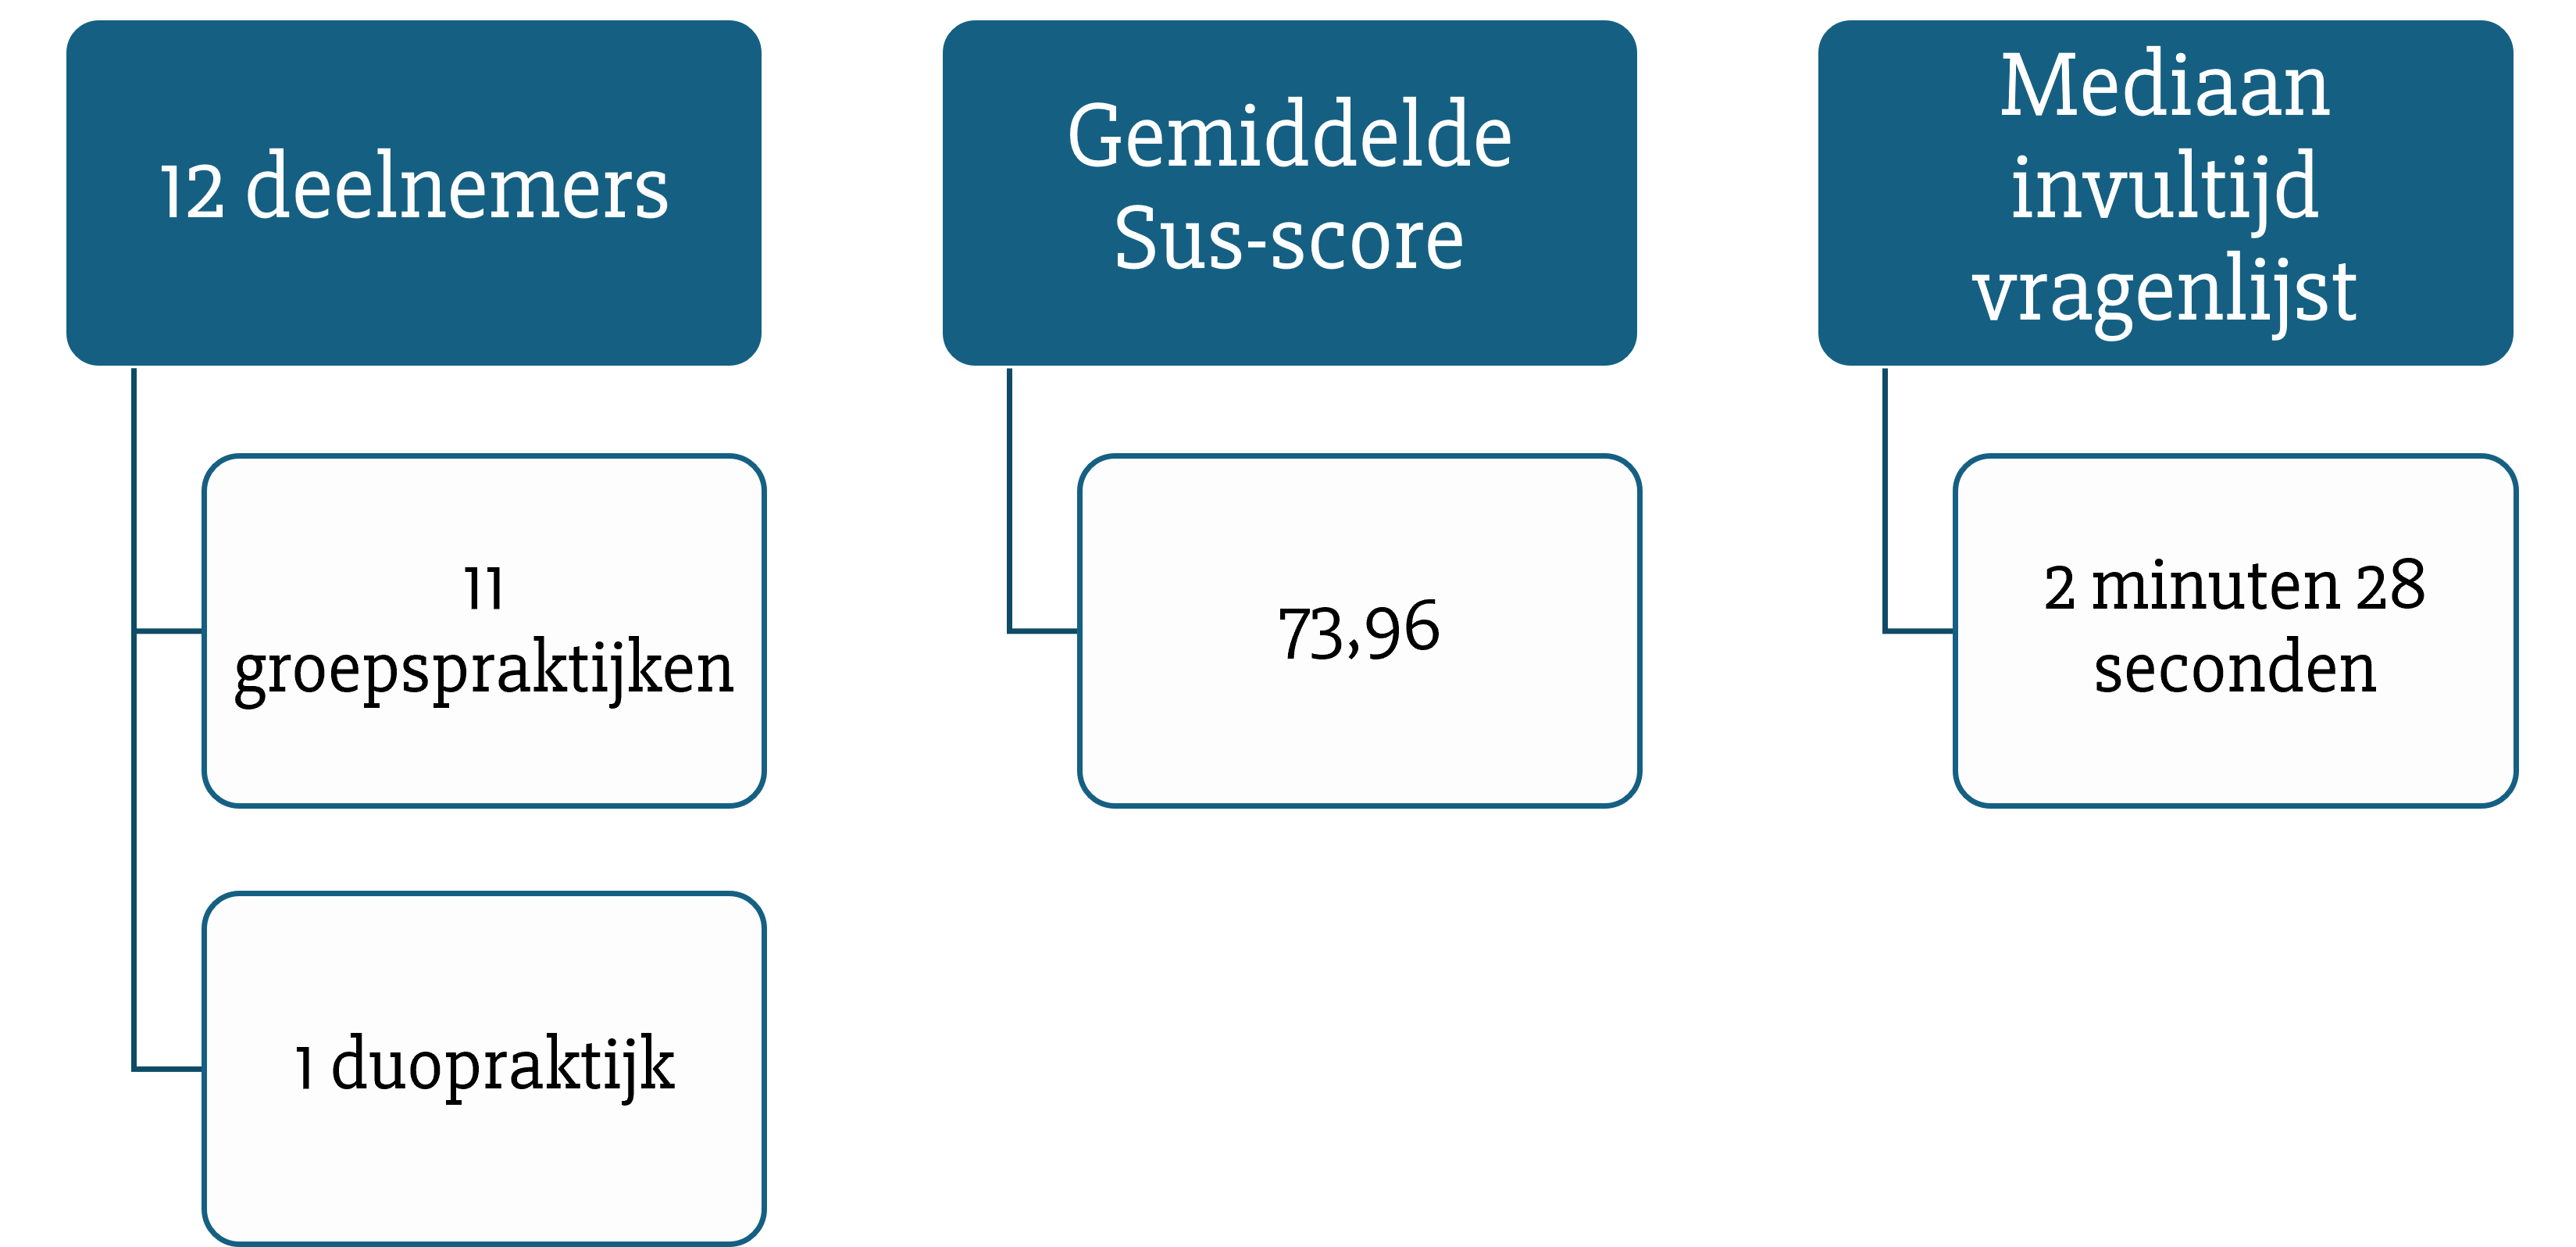
\includegraphics[width=1.0\linewidth]{graphics/Resultaten.png}
  \captionof{figure}{Overzicht van de testresultaten: SUS-score en invultijd}
\end{center}

\section{Conclusies}

De resultaten van dit onderzoek tonen aan dat een gerichte digitale interface een significante meerwaarde kan bieden bij de evaluatie van de toegankelijkheid van Vlaamse huisartsenpraktijken.
 
\begin{itemize}
  \item De SUS-score van 73,96 bevestigt dat de applicatie als \textbf{gebruiksvriendelijk} wordt ervaren
  \item De lage invultijd van 2 minuten en 28 seconden toont dat het evaluatieproces \textbf{aanzienlijk efficiënter} kan verlopen
  \item Praktijkmedewerkers gaven \textbf{positieve feedback} over de overzichtelijke opbouw en laagdrempeligheid
\end{itemize}

\section{Toekomstig onderzoek}

Op basis van de bevindingen worden de volgende vervolgstappen aanbevolen:
 
\begin{itemize}
  \item Verdere gebruikerstesten met \textbf{solo-praktijken}, om de toepasbaarheid in kleinere settings te valideren
  \item Uitbreiding met automatische \textbf{generatie van toegankelijkheidsrapporten} op basis van de ingevoerde gegevens
  \item \textbf{Integratie van aanbevelingen} dat uit de gebruikerstesten zijn gekomen
  \item Onderzoek naar de \textbf{impact op de evaluatiefrequentie} bij gebruik van de digitale tool
\end{itemize}

\end{multicols}
\end{document}